\documentclass[tikz, border=10pt]{standalone}
\usepackage{tikz}
\usepackage{amsmath}
\usepackage{amssymb}
\usetikzlibrary{shapes, arrows.meta, positioning, backgrounds, fit, calc}

% The decision stage as a learning problem: the estimator is fitted on S, the
% held-out sample V is mapped to the simplex, and the decision rule is chosen
% by empirical risk minimization on the mapped sample. Same visual language as
% figures/pipeline_diagram.tex (blue: inference, red: decision).
\begin{document}
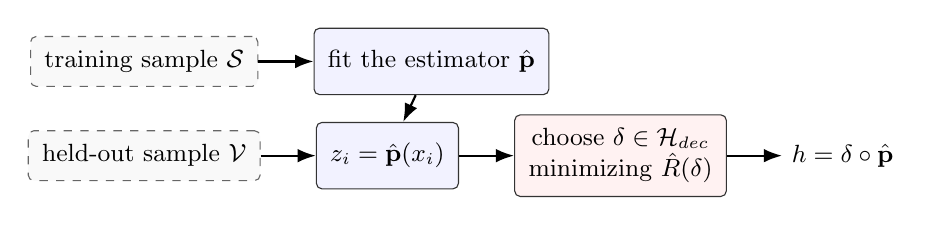
\begin{tikzpicture}[
    node distance=0.55cm and 0.7cm,
    data/.style={rectangle, draw=black!60, dashed, fill=gray!5,
      rounded corners=2pt, font=\small, inner sep=5pt, align=center},
    infer/.style={rectangle, draw=black!80, fill=blue!5, align=center,
      rounded corners=2pt, minimum height=2.4em, font=\small, inner sep=5pt},
    decide/.style={rectangle, draw=black!80, fill=red!5, align=center,
      rounded corners=2pt, minimum height=2.4em, font=\small, inner sep=5pt},
    line/.style={draw, -Latex, thick}]

  \node[data] (S) {training sample $\mathcal{S}$};
  \node[infer, right=of S] (fit) {fit the estimator $\hat{\mathbf{p}}$};

  \node[data, below=of S] (V) {held-out sample $\mathcal{V}$};
  \node[infer, right=of V] (map) {$z_i = \hat{\mathbf{p}}(x_i)$};
  \node[decide, right=of map] (erm)
    {choose $\delta \in \mathcal{H}_{dec}$\\ minimizing $\hat{R}(\delta)$};
  \node[right=of erm, font=\small] (h) {$h = \delta \circ \hat{\mathbf{p}}$};

  \path[line] (S) -- (fit);
  \path[line] (V) -- (map);
  \path[line] (fit) -- (map);
  \path[line] (map) -- (erm);
  \path[line] (erm) -- (h);
\end{tikzpicture}
\end{document}
